%%
%% This is file `tikzposter-example.tex',
%% generated with the docstrip utility.
%%
%% The original source files were:
%%
%% tikzposter.dtx  (with options: `tikzposter-example.tex')
%% 
%% This is a generated file.
%% 
%% Copyright (C) 2014 by Pascal Richter, Elena Botoeva, Richard Barnard, and Dirk Surmann
%% 
%% This file may be distributed and/or modified under the
%% conditions of the LaTeX Project Public License, either
%% version 2.0 of this license or (at your option) any later
%% version. The latest version of this license is in:
%% 
%% http://www.latex-project.org/lppl.txt
%% 
%% and version 2.0 or later is part of all distributions of
%% LaTeX version 2013/12/01 or later.
%% 
 \documentclass[20pt, a0paper, landscape, margin=0mm, innermargin=15mm,
     blockverticalspace=10mm, colspace=5mm, subcolspace=8mm]{tikzposter} %Default values for poster format options.

 \tikzposterlatexaffectionproofon %shows small comment on how the poster was made at bottom of poster
\usepackage{graphicx}
\usepackage{xpatch}
\usepackage[utf8]{inputenc}
\usepackage[english]{babel}
\usepackage[space]{grffile}
\usepackage{listings}

% Commands
 \newcommand{\bs}{\textbackslash}   % backslash
 \newcommand{\cmd}[1]{{\bf \color{red}#1}}   % highlights command


 \setlength{\tabcolsep}{2em}

 % Title, Author, Institute
 \title{\parbox{0.95\linewidth}{\centering \textbf{CODE-RADE a user centric code delivery system for science}}}
 \author{
     \begin{tabular}{c|c}
         Sean Murray & Bruce Becker
     \end{tabular}
}
\institute{Council for Scientific and Industrial Research, Meraka. University of Cape Town}
\titlegraphic{
    \raisebox{0cm}{
\includegraphics[scale=1.5]{img/coderade.png}}
    \hspace{1cm}\raisebox{-1cm}{
\includegraphics[scale=0.25]{img/CSIRlogo.jpg}}
    \hfill
    \hspace{1cm}\raisebox{-2cm}{
\includegraphics[scale=0.125]{img/UCTlogo.png}}
    \raisebox{0cm}{
\includegraphics[scale=0.2]{img/SANCG_logoTransparent-cropped.png}}
}
 % -- PREDEFINED THEMES ---------------------- %
 % Choose LAYOUT:  Default, Basic, Rays, Simple, Envelope, Wave, Board, Autumn, Desert,
\usetheme{Rays} % Board, Simple, Wave, Rays.
\usecolorstyle[colorPalette=BrownBlueOrange]{Envelope}

\defineblockstyle{BazBlock}{%
    titlewidthscale=0.8, bodywidthscale=1, titlecenter, 
    titleoffsetx=0pt, titleoffsety=0pt, bodyoffsetx=0pt, bodyoffsety=15mm,
    bodyverticalshift=15mm, roundedcorners=22, linewidth=5pt, titleinnersep=8mm,
    bodyinnersep=8mm
    }{
        \draw[rounded corners=\blockroundedcorners, inner sep=\blockbodyinnersep, line width=\blocklinewidth, color=black, top color=titlebgcolor!90, bottom color=titlebgcolor!20!white, ]
        (blockbody.south west) rectangle (blockbody.north east); %
        \ifBlockHasTitle%
        \draw[rounded corners=\blockroundedcorners, inner sep=\blocktitleinnersep, line width=\blocklinewidth, color=black, 
        top color=titlebgcolor!90, bottom color=titlebgcolor!20!white, ]
    (blocktitle.south west) rectangle (blocktitle.north east);
    \fi%    
}

\newcommand\myblock[3][BazBlock]{\useblockstyle{#1}\block{#2}{#3}\useblockstyle{Basic}}
\makeatletter
\def\TP@titlegraphictotitledistance{-5.5cm}
\settitle
{
  \centering
  \vbox
  {
    \@titlegraphic \\ [\TP@titlegraphictotitledistance] 
    \centering
    \color{titlefgcolor}
    {\bfseries \huge \sc \@title \par}
    \vspace*{1em}
    {\LARGE \@author \par}
    \vspace*{1.2em}
    {\LARGE \@institute}
  }
}

\begin{document}
\useblockstyle{Basic}
\maketitle[width=0.98\textwidth]

% basic structure
% Summary of arch and tech
% schematic of code-rade workflow, the actors etc.
% diagram of delivery 
     % map of whereit can be run (grid sites)
% description of repos and repo layouts.
% todo and next features

     \begin{columns}%blocks will be placed into columns
         \column{.25}
         \block[roundedcorners=40]{The problem CODE-RADE solves}{
             \center{The researcher is faced with a paradox.}\\
                 \center
\includegraphics[scale=.5]{img/legoparadox.png}
                 There is a huge amount of computing resources available, and a rich, well maintained, interoperable infrstructure of services... \\
             \vspace{-1cm}\center\textbf BUT \\
             Getting applictions onto it requires far too much effort.
         }         
         \block[roundedcorners=40]{CODE-RADE solves this by }{
             \begin{itemize}
                 \item Lowers barrier to entry to grid or cloud infrastructure, or single HPC site.
                 \item Application experts are able to prove to resource providers that the application will run on the sites execution environment
                 \item Easily manages the lifecycle of applications across multiple versions, architectures and configurations
                 \item Ensures that once an application is certified, its available on as many sites as possible.
                 \item Promotes collaboration between researcher, research software engineer, and infrastructure provider.
                     \item A DOI is automatically created for a version hash and deployment with pull requests as authors.
             \end{itemize}
        }
%         \block[roundedcorners=40]{7 Hypotheses of scientific computing}{
%             \begin{itemize}
%                 \item It always comes down to an application
%                 \item No software is an island
%                 \item Applications require environments.
%                 \item There are multiple environments
%                 \item Solutions decay 
%                 \item Remove humans
%                 \item Stuff is not hard, leverage what is around
%
%             \end{itemize}
%         }
         \note[targetoffsetx=-.05\textwidth,targetoffsety=9.5cm,innersep=.4cm,angle=-45,connection]{Zenodo issues a DOI}
         \block[roundedcorners=40]{CODE-RADE is }{
             \begin{itemize}
                 \item \textbf{Cross platform} It builds and test artifacts for an arbitrary set of targets, promoting diversity in computing platforms and ensures proper optimisations and application portability
                 \item \textbf{Atomic}
                                 There is fine grained control over dependencies, versions, and targets and relevant actions are taken on each event in the CODE-RADE cycle.
                                 Relevant action taken on each event of CODE-RADE cycle.
                  \item \textbf{Community}
                      No restriction is placed on the applications that can be integrated, anyone is free contribute applications(dev or testing), resource(human or hardware), code review to name a few.
                  \item \textbf{Automated}
                                 Heavy reliance on automated agents to reduce bias, lead time, and all communicated via agents in slack channels. This is a \textbf User-driven process.
             \end{itemize}

         }
         \column{0.5}
         \block[roundedcorners=40]{Workflow}{
           \center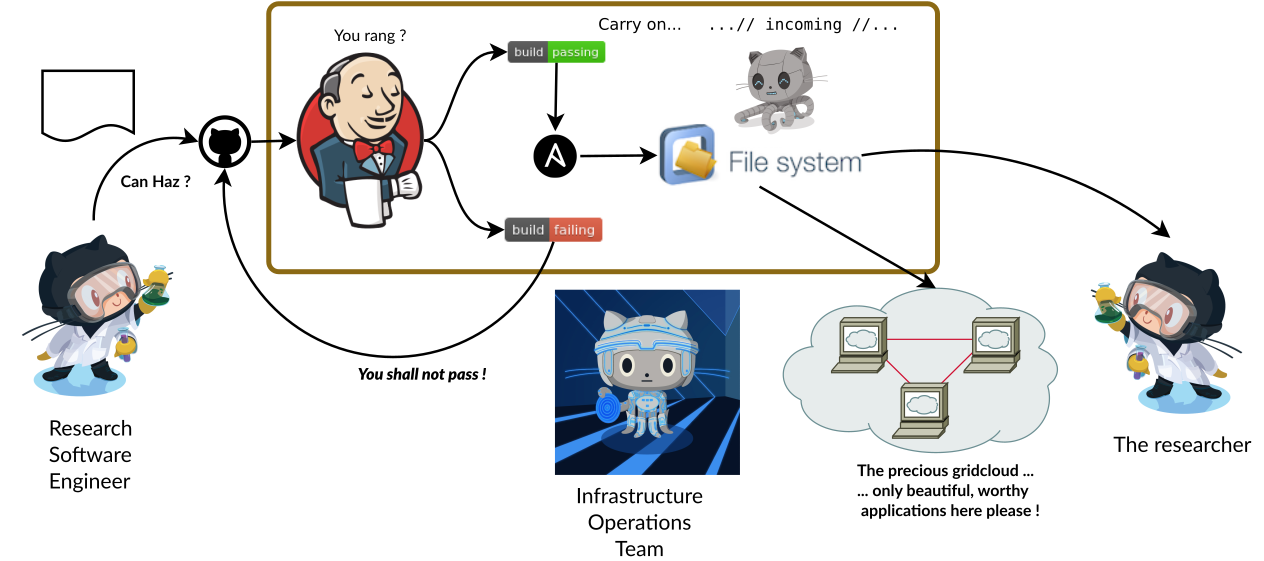
\includegraphics[scale=1]{img/code-rade-jenkins-magic.png}
         }
               \note[targetoffsetx=30cm, targetoffsety=5cm,rotate=1,angle=270,radius=8cm,width=.15\textwidth,innersep=.4cm]{                                                                     
                         At this point the hash and cvmfs release\\
                         are packaged into a DOI and the pull requesters are listed as authors.                                                                                             
                                  } 
         \begin{subcolumns}
         \subcolumn{0.5}
         \block[roundedcorners=40]{Achitecture}{
             \begin{itemize}
                     \item Components
                           \begin{itemize}
                               \item Version control at Github \textcolor{blue}{github.com/SouthAfricaDigitalScience}
                               \item Continuous Integration (Jenkins and Jarvis) \textcolor{blue}{ci.sagrid.ac.za}
                               \item Automated Delivery (CVMFS) /cvmfs/code-rade.africa-grid
                           \end{itemize}
                     \item Workflow 
                         \begin{itemize}
                                 \item Build : User and/or expert-defined means to produce executable applications or libraries
                                 \item Test : Infrastructure operator-defined targets provide a means to ensure viability
                                 \item Deliver : Ensure that once the tests pass, the application is available at all sites.
                         \end{itemize}
             \end{itemize}

         }
         \block[roundedcorners=40]{Target Matrix}{
             \begin{itemize}
                 \item One can add as many target configurations to the build matrix as can be reliably simulated.
                 \item Currently we have defined three axes :
                 \begin{itemize}
                    \item Architecture x86\_64, ARM, etc.
                    \item Operating System RHEL Ubuntu, SLES
                    \item site specific - an axis encapsulating the special nature of a site, its interconnects, compiler, local libraries, and a catch all option of generic.
                 \end{itemize} 
                     This can be seen in the directory structure of an application \\
/cvmfs/code-rade.africa-grid.org/generic/centos7/x86\_64/gcc/6.3.0
             \end{itemize}
        }
             \subcolumn{0.5}

         \block[roundedcorners=40]{Technology}{
             \begin{itemize}
                 \item docker
                 \item quay.io
                 \item persistant storage
                 \item releases get a doi, authors are submitters and PR
             \end{itemize}
        }
         \block[roundedcorners=40]{Where can all this can run}{
             %  \includegraphics{}
         }
         \end{subcolumns}
   %  \end{columns}

     % map of whereit can be run (grid sites)
% description of repos and repo layouts.
% todo and next features

     %\begin{columns}%blocks will be placed into columns
         \column{.25}

         \block[roundedcorners=40]{Repositories}{
             \begin{itemize}
                 \item I
             \end{itemize}
        }
         \block[roundedcorners=40]{Repository Layout}{
             \small\lstinputlisting{examplemodule}
         }
         \block[roundedcorners=40]{Fermionic Molecular Dynamics}{
               \begin{itemize}
                   \item \textbf{Problem Area} Nuclear physics
                   \item \textbf{Integration Time} 21 hours no prior experience
                       \begin{itemize}
                               \item github.com/SouthAfricaDigitalScience/FMD-codes-from-T.Neff-/
                                   \item ci.sagrid.ac.za/view/All/job/Fermionic-Molecular-Dynamics-deploy
                       \end{itemize}
               \end{itemize}
         }
         \block[roundedcorners=40]{Reproducibility}{
            There are two kinds of reproducibility
            \begin{itemize}
                 \item Reproducing scientific results
                     \begin{enumerate}
                         \item One should be able reproduce \textbf{exact} workflow with the \textbf{exact expression} of the application
                         \item The entire repository history is kept, allowing one to relate \textbf{each successful build} to a CVMFS repository version.
                     \end{enumerate}
                 \item Reproducing the executable application.
                     \begin{enumerate}
                         \item The \textbf{expression} of the application should be reproducible by different build systems
                         \item The means for expressing the application should be citable. This is done via Zenodo.
                     \end{enumerate}
             \end{itemize}
        }
     \end{columns}
     
     \vspace{2cm}
     \block[roundedcorners=40]{Acknowledgements}{\vspace{2em}
     %\block[titleoffsety=-1cm,bodyoffsety=-1cm]{Sample document}{\vspace{2em}
   
\includegraphics[scale=0.1]{img/UCTlogo.png}  
   \raisebox{-1cm}{
\includegraphics[scale=0.15]{img/UFSLogo.jpg}}
   \center Feedback and discussion at discourse.sci-gaia.eu
 %  \begin{flushright}
\includegraphics[scale=0.25]{img/SANCG_logoTransparent-cropped.png}\end{flushright}
     }

 \end{document}




\endinput
%%
%% End of file `tikzposter-example.tex'.
